\documentclass[11pt]{article}
\usepackage[margin=1in]{geometry}
\usepackage{graphicx}
\graphicspath{{images/}{../images/}{report/images/}}
\usepackage{listings}
\usepackage{xcolor}
\usepackage{amsmath}
\usepackage{booktabs}
\usepackage{enumitem}
\usepackage[hidelinks]{hyperref}
\usepackage{tikz}

\setcounter{tocdepth}{2}

% SystemVerilog code styling
\lstdefinestyle{verilog}{
    language=Verilog,
    basicstyle=\ttfamily\small,
    keywordstyle=\color{blue}\bfseries,
    commentstyle=\color{green!60!black},
    stringstyle=\color{red},
    numbers=left,
    numberstyle=\tiny\color{gray},
    stepnumber=1,
    numbersep=8pt,
    backgroundcolor=\color{gray!5},
    frame=single,
    breaklines=true,
    breakatwhitespace=false,
    captionpos=b,
    tabsize=2
}

\title{Project 1: MESI Cache Coherence}
\author{Sangeeth Thayaaparan \\ RIN: 662037988}
\date{\today}

\begin{document}

\maketitle

\begin{center}
  \large\textbf{Tools:} Quartus Prime 20.1.1, ModelSim - Intel FPGA Starter Edition 2020.1
\end{center}

\begin{abstract}
  This report goes over the design, implementation, and verification of a cache-coherent memory system, speficially implementing the MESI coherence protocol. The system consists of 4 processors, each with its own L1 cache, a shared L2 cache, and DRAM. The CPU testbench generates memory requests to test various scenarios (hits, misses, writebacks) and the cache controller FSM manages the state transitions to maintain coherence. More information regarding the design and verification can be found in the following sections.
\end{abstract}

\tableofcontents
\listoffigures
\listoftables

\newpage

% \vspace{0.5cm}

\section{Spec and Rationale}

The L1 caches are almost an exact copy of the cache from project 0, the specs being:

\begin{itemize}
  \item Cache Size: 512 blocks (8 KB total)
  \item Block Size: 128 bits (4 words)
  \item Address Breakdown:
        \begin{itemize}
          \item Tag: 19 bits (bits [31:13])
          \item Index: 9 bits (bits [12:4])
          \item Offset: 2 bits (bits [3:2])
        \end{itemize}
\end{itemize}

For simplicity reasons, the L2 cache is the exact same as the L1 cache. The DRAM is a simple memory model that can read/write 128-bit blocks (4 words) with single-cycle latency.

\begin{figure}[h]
  \centering
  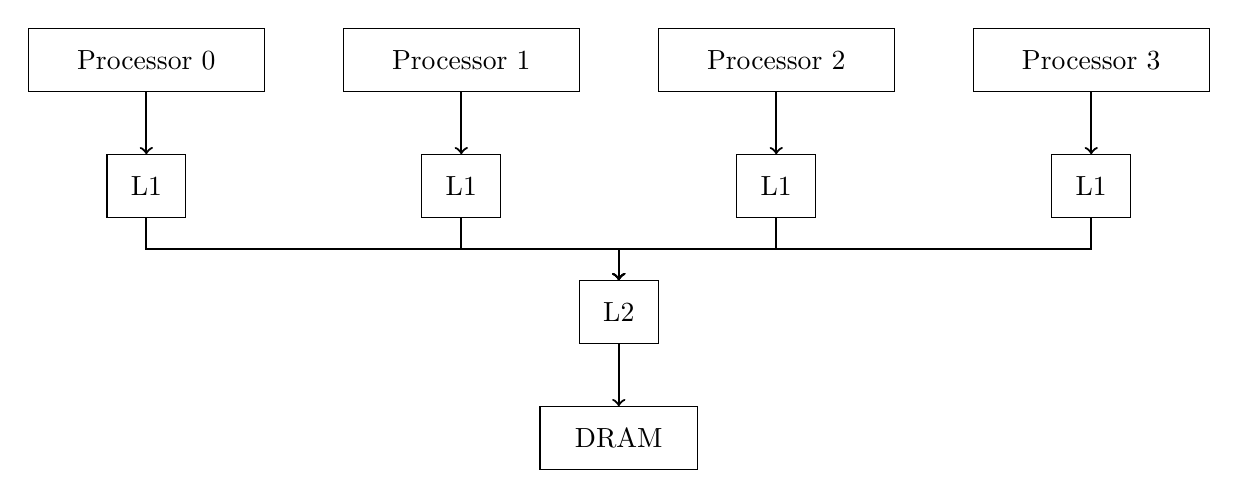
\begin{tikzpicture}
    % CPU boxes
    \draw (0, 2) rectangle (3, 2.8);
    \node at (1.5, 2.4) {Processor 0};
    \draw (4, 2) rectangle (7, 2.8);
    \node at (5.5, 2.4) {Processor 1};
    \draw (8, 2) rectangle (11, 2.8);
    \node at (9.5, 2.4) {Processor 2};
    \draw (12, 2) rectangle (15, 2.8);
    \node at (13.5, 2.4) {Processor 3};

    % L1 boxes
    \draw (1, 1.2) rectangle (2, 0.4);
    \node at (1.5, 0.8) {L1};
    \draw (5, 1.2) rectangle (6, 0.4);
    \node at (5.5, 0.8) {L1};
    \draw (9, 1.2) rectangle (10, 0.4);
    \node at (9.5, 0.8) {L1};
    \draw (13, 1.2) rectangle (14, 0.4);
    \node at (13.5, 0.8) {L1};

    % L2 box
    \draw (7, -0.4) rectangle (8, -1.2);
    \node at (7.5, -0.8) {L2};

    % DRAM box
    \draw (6.5, -2.0) rectangle (8.5, -2.8);
    \node at (7.5, -2.4) {DRAM};

    % Arrows from CPUs to L1
    \draw [->, thick] (1.5, 2) -- (1.5, 1.2);
    \draw [->, thick] (5.5, 2) -- (5.5, 1.2);
    \draw [->, thick] (9.5, 2) -- (9.5, 1.2);
    \draw [->, thick] (13.5, 2) -- (13.5, 1.2);

    % Arrows from L1 to L2 (boxy)
    \draw [->, thick] (1.5, 0.4) -- (1.5, 0) -- (7.5, 0) -- (7.5, -0.4);
    \draw [->, thick] (5.5, 0.4) -- (5.5, 0) -- (7.5, 0) -- (7.5, -0.4);
    \draw [->, thick] (9.5, 0.4) -- (9.5, 0) -- (7.5, 0) -- (7.5, -0.4);
    \draw [->, thick] (13.5, 0.4) -- (13.5, 0) -- (7.5, 0) -- (7.5, -0.4);

    % Arrow from L2 to DRAM
    \draw [->, thick] (7.5, -1.2) -- (7.5, -2.0);
  \end{tikzpicture}
  \caption{Full Cache System Block Diagram}
  \label{fig:cache_block_diagram}
\end{figure}

\section{Microarchitecture and Cycle Behavior}

\subsection{Full System Architecture Diagram}

The full system architecture was designed using KiCAD. While each module doesn't have too much to it (the inside of each subsheet just contains inputs and outputs, and the L1 cache contains multiple variants of the MESI FSM), this schematic was mostly used to help design the verilog code. Specifically picking and choosing the names of each wires and how the modules are connected together. While the final verilog code modifies some of the names (as there are various repeat names for different lines and buses), the overal structure of the system was based off this schematic.

\newpage

% Picture of the kicad screenshot showing the full stuff
\begin{figure}[!h]
  \centering
  \includegraphics[width=\textwidth]{images/MESITopLevelArch/CacheHierarchy.pdf}
  \caption{Full System Architecture Diagram (created by author).}
  \label{fig:full_system_architecture}
\end{figure}

\subsection{Module Descriptions}

\subsubsection{Module: CPU}

\paragraph{Behavior:}
The \texttt{cpu} module isn't actually implemented as it's own module in the verilog code. Rather, the testbench generates the CPU requests directly. The CPU generates memory requests with an address, data, read/write signal, and a \textit{valid} signal. It waits for the cache to assert \texttt{Ready} before issuing the next request. Correctness means: all test vectors are issued in order and the CPU properly waits for completion.

Key signals:
\begin{itemize}[noitemsep, label={--}]
  \item \texttt{Valid} (1 bit, output): Indicates a new request is being issued
  \item \texttt{DataAdr} (32 bits, output): Address for the memory operation
  \item \texttt{WriteData} (32 bits, output): Data to write (for write operations)
  \item \texttt{MemWrite} (1 bit, output): 1 for write, 0 for read
  \item \texttt{Ready} (1 bit, input): Asserted by cache when request is complete
\end{itemize}

\paragraph{Key State:}
\begin{itemize}[noitemsep, label={--}]
  \item \texttt{testvectors[0:99]}: Array of test vectors loaded from file, each containing \{address, data, write\}
  \item \texttt{vectornum}: Index of the current test vector being issued
\end{itemize}

\paragraph{Implementation:} \leavevmode \\
\begin{lstlisting}[style=verilog, caption=Test Vector Format (from testbench)]
typedef struct {
  logic [31:0]  addr;
  logic         write;
  logic [1:0]   l1_id;
  logic [31:0]  data;
  int           cycle;
} test_vector_t;
\end{lstlisting}

\begin{lstlisting}[style=verilog, caption=Cycle-Based Request Issue (from testbench)]
for (int cycle = 0; cycle <= max_cycle; cycle++) begin
  test_vector_t pending_vectors[$];
  pending_vectors = vectors_by_cycle[cycle];

  if (pending_vectors.size() > 0) begin
    for (int l1 = 0; l1 < 4; l1++) dut.l1_valid[l1] = 1'b0;

    foreach (pending_vectors[i]) begin
      issue_request(pending_vectors[i]);
    end

    wait_for_all_ready(pending_vectors, max_cycle, cycle);
  end
end
\end{lstlisting}

\begin{lstlisting}[style=verilog, caption=Per-Request Completion Handling (from testbench)]
task automatic wait_for_all_ready(ref test_vector_t pending_vectors[$],
                                  input int max_cycle,
                                  input int current_cycle);
  int done_count = 0;
  int total_count = pending_vectors.size();
  bit ready_mask[];

  ready_mask = new[total_count];
  @(posedge clk);

  while (done_count < total_count) begin
    done_count = 0;
    foreach (pending_vectors[i]) begin
      if (!ready_mask[i] && dut.l1_ready[pending_vectors[i].l1_id]) begin
        ready_mask[i] = 1'b1;
        dut.l1_valid[pending_vectors[i].l1_id] = 1'b0;
      end
      if (ready_mask[i]) done_count++;
    end
    if (done_count < total_count) @(posedge clk);
  end
endtask
\end{lstlisting}


\subsubsection{Module: L1 cache}

\paragraph{Behavior:}
The \texttt{L1} module is a direct-mapped private cache for each processor with MESI coherence states (\texttt{INVALID/SHARED/EXCLUSIVE/MODIFIED}). It accepts CPU read/write requests, serves hits locally, and issues bus transactions on misses or upgrades (\texttt{BusRd}, \texttt{BusRdX}, \texttt{BusUpgr}). It also snoops peer transactions and performs coherence state transitions plus invalidations as needed.

Key signals:
\begin{itemize}[noitemsep, label={--}]
  \item \texttt{Valid}, \texttt{MemWrite}, \texttt{DataAdr}, \texttt{WriteData}: CPU-side request interface
  \item \texttt{ReadData}, \texttt{Ready}, \texttt{CacheHit}: CPU-side response/status interface
  \item \texttt{BusReq}, \texttt{BusGrant}: arbitration handshake
  \item \texttt{Data}, \texttt{BusAdr}, \texttt{BusOp}, \texttt{BusValid}, \texttt{BusShared}, \texttt{BusBusy}: shared coherence bus
\end{itemize}

\paragraph{Key State:}
\begin{itemize}[noitemsep, label={--}]
  \item \texttt{SRAM[511:0]}: cache lines with MESI state, dirty bit, tag, and 128-bit block data
  \item \texttt{ctrl\_state}: transaction controller FSM (\texttt{IDLE}, \texttt{REQUEST\_BUFFERED}, \texttt{MISS\_PENDING}, \texttt{BUS\_ACTIVE}, \texttt{WRITEBACK\_PENDING})
  \item Buffered request registers (\texttt{req\_addr}, \texttt{req\_wdata}, \texttt{req\_write}, \texttt{req\_valid}) and writeback buffer (\texttt{wb\_addr}, \texttt{wb\_data}, \texttt{wb\_pending})
\end{itemize}

\paragraph{Implementation:} \leavevmode \\
\begin{lstlisting}[style=verilog, caption=L1 MESI + Controller States]
typedef enum logic [1:0] {
  INVALID,
  SHARED,
  EXCLUSIVE,
  MODIFIED
} mesi_t;

typedef enum logic [2:0] {
  IDLE,
  REQUEST_BUFFERED,
  MISS_PENDING,
  BUS_ACTIVE,
  WRITEBACK_PENDING
} ctrl_t;
\end{lstlisting}

\begin{lstlisting}[style=verilog, caption=L1 Hit Detection and Hit/Miss Path]
assign cache_hit_comb = req_valid &&
                        (SRAM[req_index].mesi_state != INVALID) &&
                        (SRAM[req_index].tag == req_tag);

REQUEST_BUFFERED: begin
  if (cache_hit_comb) begin
    CacheHit = 1'b1;
    if (req_write && SRAM[req_index].mesi_state == SHARED) begin
      ctrl_next = MISS_PENDING; // upgrade via bus
      BusReq = 1'b1;
    end else begin
      Ready = 1'b1;
      ctrl_next = IDLE;
    end
  end else begin
    ctrl_next = (SRAM[req_index].dirty && SRAM[req_index].mesi_state != INVALID)
                ? WRITEBACK_PENDING : MISS_PENDING;
  end
end
\end{lstlisting}


\subsubsection{Module: L2 cache}

\paragraph{Behavior:}
The \texttt{L2} module is a shared inclusive cache and coherence responder on the bus. It snoops \texttt{BusRd/BusRdX/BusUpgr/Writeback}, returns data on L2 hits, triggers DRAM reads on L2 misses, and installs/updates returned lines. It also tracks sharer information and can assert \texttt{BusShared}.

Key signals:
\begin{itemize}[noitemsep, label={--}]
  \item \texttt{Data}, \texttt{BusAdr}, \texttt{BusOp}, \texttt{BusValid}, \texttt{BusShared}, \texttt{BusBusy}: shared coherence bus interface
  \item \texttt{dram\_valid}, \texttt{dram\_write}, \texttt{dram\_addr}, \texttt{dram\_wdata}: DRAM request interface
  \item \texttt{dram\_rdata}, \texttt{dram\_ready}: DRAM response interface
\end{itemize}

\paragraph{Key State:}
\begin{itemize}[noitemsep, label={--}]
  \item \texttt{L2\_SRAM[511:0]}: valid/tag/sharer mask/data per cache line
  \item DRAM miss tracking: \texttt{dram\_pending}, \texttt{dram\_pending\_tag}, \texttt{dram\_pending\_index}, \texttt{dram\_pending\_busadr}
\end{itemize}

\paragraph{Implementation:} \leavevmode \\
\begin{lstlisting}[style=verilog, caption=L2 Line Format and DRAM Miss Path]
typedef struct packed {
  logic        valid;
  logic [18:0] tag;
  logic [3:0]  l1_sharers;
  logic [127:0] data;
} l2_block_t;

if (BusOp === 3'b000 || BusOp === 3'b001) begin
  if (L2_SRAM[bus_index].valid && L2_SRAM[bus_index].tag == bus_tag) begin
    data_out = L2_SRAM[bus_index].data;
    data_oe = 1'b1;
    busvalid_out = 1'b1;
  end else begin
    dram_valid = 1'b1;
    dram_write = 1'b0;
    dram_addr = {BusAdr[31:4], 4'b0000};
  end
end
\end{lstlisting}

\begin{lstlisting}[style=verilog, caption=L2 DRAM Fill and Bus Update]
if (dram_pending && dram_ready) begin
  L2_SRAM[dram_pending_index].valid <= 1'b1;
  L2_SRAM[dram_pending_index].tag <= dram_pending_tag;
  L2_SRAM[dram_pending_index].data <= dram_rdata;
  dram_pending <= 1'b0;
end

if (BusOp === 3'b011 && !$isunknown(Data)) begin // Writeback
  L2_SRAM[bus_index].valid <= 1'b1;
  L2_SRAM[bus_index].tag <= bus_tag;
  L2_SRAM[bus_index].data <= Data;
end
\end{lstlisting}


\subsubsection{Module: dram}

\paragraph{Behavior:}
The \texttt{dram} module models backing main memory using a 32-bit word array and supports 128-bit block transfers (4 consecutive words) for cache-line fills and writebacks. On \texttt{Valid}, it performs either a block write or block read and asserts \texttt{Ready}.

Key signals:
\begin{itemize}[noitemsep, label={--}]
  \item \texttt{Valid}: transaction request
  \item \texttt{MemWrite}: write/read select
  \item \texttt{DataAdr}: starting word address
  \item \texttt{WriteDataBlock}, \texttt{ReadDataBlock}: 128-bit block data interface
  \item \texttt{Ready}: transaction complete
\end{itemize}

\paragraph{Key State:}
\begin{itemize}[noitemsep, label={--}]
  \item \texttt{DRAM[1048575:0]}: 1,048,576-word memory array (32-bit words)
\end{itemize}

\paragraph{Implementation:} \leavevmode \\
\begin{lstlisting}[style=verilog, caption=DRAM Block Read/Write Logic]
always @(posedge clk) begin
  if (Valid) begin
    if (MemWrite) begin
      DRAM[DataAdr]     <= WriteDataBlock[31:0];
      DRAM[DataAdr + 1] <= WriteDataBlock[63:32];
      DRAM[DataAdr + 2] <= WriteDataBlock[95:64];
      DRAM[DataAdr + 3] <= WriteDataBlock[127:96];
    end else begin
      ReadDataBlock[31:0]   <= DRAM[DataAdr];
      ReadDataBlock[63:32]  <= DRAM[DataAdr + 1];
      ReadDataBlock[95:64]  <= DRAM[DataAdr + 2];
      ReadDataBlock[127:96] <= DRAM[DataAdr + 3];
    end
    Ready <= 1;
  end else begin
    Ready <= 0;
  end
end
\end{lstlisting}


\subsubsection{Module: Arbiter}

\paragraph{Behavior:}
The \texttt{Arbiter} module grants bus ownership among the 4 L1 caches using round-robin priority. It preserves ownership while the current owner continues requesting and selects the next requester when the bus is released.

Key signals:
\begin{itemize}[noitemsep, label={--}]
  \item \texttt{BusReq[3:0]}: bus requests from L1-0..L1-3
  \item \texttt{BusGrant[3:0]}: one-hot bus grant output
  \item \texttt{BusBusy}: shared busy line (tri-stated by arbiter, driven by bus users)
\end{itemize}

\paragraph{What is Round Robin?}

It's an arbitration scheme that cycles through requesters in a fixed order, granting access to the next requester in line after the current one finishes. This scheme is also used in various other places regarding computers, such as process scheduling in operating systems.

\begin{figure}[h]
  \centering
  \includegraphics[width=0.6\textwidth]{images/rr.png}
  \caption{Round-robin arbitration illustration (adapted from \protect\cite{cs341-scheduling}).}
  \label{fig:round_robin}
\end{figure}

Essentially it loops through the requesters in a circle.

\paragraph{Key State:}
\begin{itemize}[noitemsep, label={--}]
  \item \texttt{grant\_pointer}: round-robin starting priority pointer
  \item \texttt{grant\_reg}/\texttt{grant\_next}: current and next one-hot grant state
\end{itemize}

\paragraph{Implementation:} \leavevmode \\
\begin{lstlisting}[style=verilog, caption=Round-Robin Grant Selection]
always_comb begin
  grant_next = grant_reg;

  if (|grant_reg) begin
    if ((grant_reg & BusReq) == 4'b0000) begin
      grant_next = 4'b0000;
    end
  end

  if (grant_next == 4'b0000) begin
    for (int i = 0; i < 4; i = i + 1) begin
      if (BusReq[(grant_pointer + i[1:0]) & 2'b11] && grant_next == 4'b0000)
        grant_next[(grant_pointer + i[1:0]) & 2'b11] = 1'b1;
    end
  end
end
\end{lstlisting}

\begin{lstlisting}[style=verilog, caption=Grant Register and Pointer Update]
always_ff @(posedge clk) begin
  if (reset) begin
    grant_pointer <= 2'b00;
    grant_reg <= 4'b0000;
  end else begin
    grant_reg <= grant_next;
    if (grant_reg == 4'b0000 && grant_next != 4'b0000) begin
      for (int i = 0; i < 4; i = i + 1)
        if (grant_next[i]) grant_pointer <= i[1:0] + 2'b01;
    end
  end
end
\end{lstlisting}

\section{Verification and Results}

% Purpose

\subsubsection{Purpose}

There are 5 main tests that are being accounted for in this implementation:
\begin{itemize}[noitemsep, label={--}]
  \item Single processor reads
  \item Single processor writes
  \item Cache coherence
  \item Arbitration
  \item Memory eviction
\end{itemize}

These tests inadvertently cover a lot of different scenarios, such as:
\begin{itemize}[noitemsep, label={--}]
  \item Cache hits and misses
  \item Writebacks of dirty blocks
  \item Coherence state transitions (e.g. SHARED to MODIFIED on write)
  \item Bus transactions (BusRd, BusRdX, BusUpgr)
  \item DRAM interactions on L2 misses
\end{itemize}

This state transition diagram is what our MESI model should be following:

\newpage

\begin{figure}[h]
  \centering
  \includegraphics[width=0.5\textwidth]{images/Diagrama_MESI.png}
  \caption{MESI state transition diagram (from \protect\cite{wiki-mesi}, credited to \protect\cite{culler1997}).}
  \label{fig:mesi_diagram}
\end{figure}

% Stimulus

\subsection{Test 1: Memory Read}

This test ensures that memory is being loaded correctly into each cache block.
\textit{Stimulus file: Listing~\ref{lst:test1_vectors} (Appendix~\ref{sec:appendix_test_vectors}).}

% 00000000_0_0_00000000_0
% 00000004_0_0_00000000_1
% 00000008_0_0_00000000_2
% 0000000C_0_0_00000000_3
% 00000100_0_1_00000000_4
% 00000104_0_2_00000000_5
% 00000108_0_3_00000000_6

% \enlargethispage{2\baselineskip} % gives this page a little extra vertical room

\begin{table}[!htbp]
  \centering
  \footnotesize
  \setlength{\tabcolsep}{3.5pt}      % tighter columns
  \renewcommand{\arraystretch}{0.94} % tighter row height
  \caption{Test 1 (Memory Read): stimulus and expected cache/coherence behavior}
  \label{tab:test1_memory_read}
  \begin{tabular}{@{}c c c c p{8.8cm}@{}}
    \toprule
    Cycle & Address    & Op   & Req. & Expected behavior                                             \\
    \midrule
    0     & 0x00000000 & Read & L1-0 & Cold miss; BusRd; fill line \{0x00,0x04,0x08,0x0C\}.          \\
    1     & 0x00000004 & Read & L1-0 & Same line as cycle 0; hit (offset change only).               \\
    2     & 0x00000008 & Read & L1-0 & Same line; hit.                                               \\
    3     & 0x0000000C & Read & L1-0 & Same line; hit.                                               \\
    4     & 0x00000100 & Read & L1-1 & New line for L1-1; miss and fill expected.                    \\
    5     & 0x00000104 & Read & L1-2 & Same line family as cycle 4; shared copy behavior expected.   \\
    6     & 0x00000108 & Read & L1-3 & Same shared line family; shared-state behavior remains valid. \\
    \bottomrule
  \end{tabular}
\end{table}

\newpage

\subsubsection{Waveforms}

\begin{figure}[!htbp]
  \centering
  \includegraphics[width=\textwidth]{images/Test1_waveforms.png}
  \caption{Test 1 waveform showing memory read operations, cache hits/misses, and MESI state transitions.}
  \label{fig:test1_waveforms}
\end{figure}

Given the waveforms, there are some imporant things to note to know that the test is working correctly:

\begin{itemize}[noitemsep, label={--}]
  \item \texttt{l1\_cache\_hit} is 0 for the first request, but changes values for the next 3 requests. It's not visible in the image, but it does change its value to 1 for the next 3 requests, which means that those are hits.
  \item The MESI state for the first request changes to EXCLUSIVE, and then changes to SHARED for the next 3 requests, which is expected since the first request is a cold miss, and the next 3 requests are hits to the same line, which should be in SHARED state since multiple caches have a copy of the same line.
  \item The bus transactions for the first request is a BusRd, which is expected since it's a miss. The next 3 requests don't have any bus transactions, which is expected since they are hits.
\end{itemize}

% // Test 2: Single writes with 32-bit data
% // Each write completes before next one starts (different cycles)
% // ADDRESS_MEMWRITE_L1ID_DATA_CYCLE
% 00000010_1_0_DEADBEEF_0
% 00000014_1_0_BEDFACED_1
% 00000020_1_1_AAAABBBB_2
% 00000024_1_2_CCCCDDDD_3
% 00000028_1_3_EEEEAAAA_4

\subsection{Test 2: Memory Write}

This test checks single-core and multi-core write behavior, including write misses, ownership acquisition, and dirty-line updates.
\textit{Stimulus file: Listing~\ref{lst:test2_vectors} (Appendix~\ref{sec:appendix_test_vectors}).}

\begin{table}[!htbp]
  \centering
  \footnotesize
  \setlength{\tabcolsep}{3.5pt}
  \renewcommand{\arraystretch}{0.94}
  \caption{Test 2 (Memory Write): stimulus and expected cache/coherence behavior}
  \label{tab:test2_memory_write}
  \begin{tabular}{@{}c c c c c p{7.1cm}@{}}
    \toprule
    Cycle & Address    & Op    & Req. & Data       & Expected behavior                                                                              \\
    \midrule
    0     & 0x00000010 & Write & L1-0 & 0xDEADBEEF & Write miss; BusRdX (or write-allocate path); line filled, word updated, line becomes MODIFIED. \\
    1     & 0x00000014 & Write & L1-0 & 0xBEDFACED & Same cache line family as prior access; write hit in owned line, remains MODIFIED.             \\
    2     & 0x00000020 & Write & L1-1 & 0xAAAABBBB & Independent write by another core; miss + ownership acquisition expected for L1-1 line.        \\
    3     & 0x00000024 & Write & L1-2 & 0xCCCCDDDD & Miss for L1-2 on its line; BusRdX/fill/update expected.                                        \\
    4     & 0x00000028 & Write & L1-3 & 0xEEEEAAAA & Miss for L1-3 on its line; data written and line ends MODIFIED.                                \\
    \bottomrule
  \end{tabular}
\end{table}

\subsubsection{Waveforms}

\begin{figure}[!htbp]
  \centering
  \includegraphics[width=\textwidth]{images/Test2_waveforms.png}
  \caption{Test 2 waveform showing memory write operations, cache hits/misses, MESI state transitions, and bus transactions.}
  \label{fig:test2_waveforms}
\end{figure}

\begin{itemize}[noitemsep, label={--}]
  \item First write to each new line should show miss behavior (bus transaction present).
  \item Re-write within an already-owned line should avoid refill and complete as a hit.
  \item Updated word lane in cache line should match written data values.
\end{itemize}

% // Test 3: Coherence scenario - snooping initiated MESI state transitions
% // ADDRESS_MEMWRITE_L1ID_DATA_CYCLE
% // Scenario 1 (Cycle 0): Both L1s read same address (both should reach SHARED state)
% // Concurrent reads on same cycle to test snoop response
% 00000200_0_0_00000000_0
% 00000200_0_1_00000000_0
% // Scenario 2 (Cycle 1-3): L1-0 reads, L1-1 writes (upgrading invalidates others)
% // Sequential to show state transition
% 00000204_0_0_00000000_1
% 00000204_1_1_FFFFFFFF_2
% 00000204_0_0_00000000_3
% // Scenario 3 (Cycle 4-5): Multi-L1 coherence - read-then-write pattern
% // Both read concurrently, then L1-0 writes (invalidates L1-1's copy)
% 00000208_0_0_00000000_4
% 00000208_0_1_00000000_4
% 00000208_1_0_99999999_5

\subsection{Test 3: Cache Coherence (Snooping + MESI Transitions)}

This test validates snoop-driven coherence behavior across L1 caches, including SHARED formation, invalidation on write, and read-after-invalidate correctness.
\textit{Stimulus file: Listing~\ref{lst:test3_vectors} (Appendix~\ref{sec:appendix_test_vectors}).}

\begin{table}[!htbp]
  \centering
  \footnotesize
  \setlength{\tabcolsep}{3.5pt}
  \renewcommand{\arraystretch}{0.94}
  \caption{Test 3 (Cache Coherence): stimulus and expected cache/coherence behavior}
  \label{tab:test3_cache_coherence}
  \begin{tabular}{@{}c c c c c p{6.8cm}@{}}
    \toprule
    Cycle & Address    & Op    & Req. & Data       & Expected behavior                                                                                    \\
    \midrule
    0     & 0x00000200 & Read  & L1-0 & 0x00000000 & Concurrent read with L1-1 to same line; first reader may fetch, both should converge to SHARED.      \\
    0     & 0x00000200 & Read  & L1-1 & 0x00000000 & Snoop/BusShared path active; both caches hold coherent shared copies after fill/response.            \\
    1     & 0x00000204 & Read  & L1-0 & 0x00000000 & L1-0 reads line first (E/S depending on sharers).                                                    \\
    2     & 0x00000204 & Write & L1-1 & 0xFFFFFFFF & L1-1 write requires ownership (BusRdX/BusUpgr); peer shared copy invalidated; L1-1 becomes MODIFIED. \\
    3     & 0x00000204 & Read  & L1-0 & 0x00000000 & L1-0 re-read after invalidation must miss/refetch; returned data should reflect L1-1 write.          \\
    4     & 0x00000208 & Read  & L1-0 & 0x00000000 & Concurrent read pair with L1-1 creates shared line in both caches.                                   \\
    4     & 0x00000208 & Read  & L1-1 & 0x00000000 & Shared-state confirmation via snoop-visible bus behavior.                                            \\
    5     & 0x00000208 & Write & L1-0 & 0x99999999 & Writer upgrades/gets ownership; other sharer invalidated; writer ends MODIFIED.                      \\
    \bottomrule
  \end{tabular}
\end{table}

\subsubsection{Waveforms}

\begin{figure}[!htbp]
  \centering
  \includegraphics[width=\textwidth]{images/Test3_waveforms.png}
  \caption{Test 3 waveform showing coherence snoops, shared-line formation, invalidation, and ownership transfer.}
  \label{fig:test3_waveforms}
\end{figure}

\begin{itemize}[noitemsep, label={--}]
  \item Concurrent reads to the same address should show shared-copy behavior (BusShared/snoop-visible response).
  \item Write from one cache to a shared line should invalidate peer copies and transition writer to MODIFIED.
  \item Read-after-invalidate should miss and return updated data.
\end{itemize}


% // Test 4: Arbitration - concurrent requests from all 4 L1s
% // Format: ADDRESS_MEMWRITE_L1ID_DATA_CYCLE
% // 
% // KEY TIMING CONCEPT:
% // - Cycle 0: All 4 reads issued SIMULTANEOUSLY (concurrent)
% //   The arbiter grants them one-by-one in round-robin order
% // - Cycle 10: All 4 writes issued SIMULTANEOUSLY (concurrent, delayed)
% //
% // Round 1 (Cycle 0): CONCURRENT reads - arbiter tests round-robin
% 00000300_0_0_00000000_0
% 00000304_0_1_00000000_0
% 00000308_0_2_00000000_0
% 0000030C_0_3_00000000_0
% // Round 2 (Cycle 10): CONCURRENT writes - arbiter tests round-robin
% 00000310_1_0_AAAAAAAA_10
% 00000314_1_1_BBBBBBBB_10
% 00000318_1_2_CCCCCCCC_10
% 0000031C_1_3_DDDDDDDD_10

\subsection{Test 4: Arbitration (Round-Robin Fairness Under Contention)}

This test verifies that simultaneous requests from all four L1 caches are granted in fair round-robin order for both read and write bursts.
\textit{Stimulus file: Listing~\ref{lst:test4_vectors} (Appendix~\ref{sec:appendix_test_vectors}).}

\begin{table}[!htbp]
  \centering
  \footnotesize
  \setlength{\tabcolsep}{3.5pt}
  \renewcommand{\arraystretch}{0.94}
  \caption{Test 4 (Arbitration): concurrent request groups and expected arbiter behavior}
  \label{tab:test4_arbitration}
  \begin{tabular}{@{}c c c c c p{6.8cm}@{}}
    \toprule
    Cycle & Address    & Op    & Req. & Data       & Expected behavior                                                                                \\
    \midrule
    0     & 0x00000300 & Read  & L1-0 & 0x00000000 & All four reads arrive together; grants should serialize in round-robin order without starvation. \\
    0     & 0x00000304 & Read  & L1-1 & 0x00000000 & Request remains pending until granted; BusGrant should be one-hot each service window.           \\
    0     & 0x00000308 & Read  & L1-2 & 0x00000000 & Arbiter rotates priority pointer after each completed ownership window.                          \\
    0     & 0x0000030C & Read  & L1-3 & 0x00000000 & Final requester in first contention group must still be serviced correctly.                      \\
    10    & 0x00000310 & Write & L1-0 & 0xAAAAAAAA & Second contention group (writes): same fairness behavior expected under write traffic.           \\
    10    & 0x00000314 & Write & L1-1 & 0xBBBBBBBB & One-hot grant + no overlap on bus ownership.                                                     \\
    10    & 0x00000318 & Write & L1-2 & 0xCCCCCCCC & Each requester eventually receives grant; no livelock/starvation.                                \\
    10    & 0x0000031C & Write & L1-3 & 0xDDDDDDDD & Rotation should continue consistently from prior pointer state.                                  \\
    \bottomrule
  \end{tabular}
\end{table}

\subsubsection{Waveforms}

\begin{figure}[!htbp]
  \centering
  \includegraphics[width=\textwidth]{images/Test4_waveforms.png}
  \caption{Test 4 waveform showing concurrent requests and round-robin bus grant sequencing.}
  \label{fig:test4_waveforms}
\end{figure}

\begin{itemize}[noitemsep, label={--}]
  \item For each contention burst, \texttt{BusGrant[3:0]} should be one-hot and rotate fairly.
  \item \texttt{BusBusy} should remain asserted while an owner is active, then release for next grant.
  \item All four requesters in each burst should complete with no starvation.
\end{itemize}

% // Test 5: Cache line eviction and write-back
% // ADDRESS_MEMWRITE_L1ID_DATA_CYCLE
% // Addresses with same index but different tags (direct-mapped cache)
% // This tests write-back buffer and dirty line eviction
% // SEQUENTIAL execution: each write must complete before next starts

% // Step 1 (Cycle 0): Write to address 0x00000000
% 00000000_1_0_AAAAAAAA_0

% // Step 2 (Cycle 1): Write to address 0x00002000 (different tag, same index, evicts prev)
% 00002000_1_0_BBBBBBBB_1

% // Step 3 (Cycle 2): Write to address 0x00004000 (evicts second line)
% 00004000_1_0_CCCCCCCC_2

% // Step 4 (Cycle 3): Read from address 0x00000000 (should miss, line was evicted)
% 00000000_0_0_00000000_3

% // Step 5 (Cycle 4-5): Test eviction with different L1s
% 00006000_1_1_DDDDDDDD_4
% 00008000_1_1_EEEEEEEE_5

\subsection{Test 5: Memory Eviction and Writeback}

This test validates direct-mapped conflict eviction, dirty-line writeback, and correct data recovery after eviction.
\textit{Stimulus file: Listing~\ref{lst:test5_vectors} (Appendix~\ref{sec:appendix_test_vectors}).}

\begin{table}[!htbp]
  \centering
  \footnotesize
  \setlength{\tabcolsep}{3.5pt}
  \renewcommand{\arraystretch}{0.94}
  \caption{Test 5 (Eviction/Writeback): stimulus and expected behavior}
  \label{tab:test5_eviction_writeback}
  \begin{tabular}{@{}c c c c c p{6.8cm}@{}}
    \toprule
    Cycle & Address    & Op    & Req. & Data       & Expected behavior                                                                                   \\
    \midrule
    0     & 0x00000000 & Write & L1-0 & 0xAAAAAAAA & Write miss/fill then update; line in L1-0 becomes MODIFIED (dirty).                                 \\
    1     & 0x00002000 & Write & L1-0 & 0xBBBBBBBB & Same index, different tag: dirty victim eviction; writeback expected before/with replacement.       \\
    2     & 0x00004000 & Write & L1-0 & 0xCCCCCCCC & Another conflict on same index: second eviction/writeback path exercised.                           \\
    3     & 0x00000000 & Read  & L1-0 & 0x00000000 & Re-read original line should miss (evicted) and fetch most recent committed value from lower level. \\
    4     & 0x00006000 & Write & L1-1 & 0xDDDDDDDD & Repeat eviction behavior on a different core; verifies per-core buffer/control path.                \\
    5     & 0x00008000 & Write & L1-1 & 0xEEEEEEEE & Conflict replacement in L1-1 triggers dirty handling consistently.                                  \\
    \bottomrule
  \end{tabular}
\end{table}

\subsubsection{Waveforms}

\begin{figure}[!htbp]
  \centering
  \includegraphics[width=\textwidth]{images/Test5_waveforms.png}
  \caption{Test 5 waveform showing conflict misses, dirty evictions, writeback transactions, and reload behavior.}
  \label{fig:test5_waveforms}
\end{figure}

\begin{itemize}[noitemsep, label={--}]
  \item Conflict addresses mapping to the same index should trigger eviction/replacement.
  \item Dirty victim lines should generate writeback traffic before data loss.
  \item Post-eviction read should miss and return the correct committed value.
  \item It's unable to see the writeback transactions in the waveform, but they do happen in the simulation, which can be verified by looking at the L2 and DRAM interactions, and how the L2 line changes at the evicting address.
\end{itemize}

% \lstinputlisting[language=, caption=Test Vectors from cache\_test.txt]{../cache_test.tv}

% Expected Result

\clearpage
\appendix
\section{Test Vector Files}
\label{sec:appendix_test_vectors}

\subsection{Test 1 Vectors (Memory Read)}
\lstinputlisting[
  style=verilog,
  caption={Test 1 vectors: \texttt{test1.single\_read.txt}},
  label={lst:test1_vectors}
]{../tests/test1.single_read.txt}

\subsection{Test 2 Vectors (Memory Write)}
\lstinputlisting[
  style=verilog,
  caption={Test 2 vectors: \texttt{test2.single\_write.txt}},
  label={lst:test2_vectors}
]{../tests/test2.single_write.txt}

\subsection{Test 3 Vectors (Cache Coherence)}
\lstinputlisting[
  style=verilog,
  caption={Test 3 vectors: \texttt{test3.coherence.txt}},
  label={lst:test3_vectors}
]{../tests/test3.coherence.txt}

\subsection{Test 4 Vectors (Arbitration)}
\lstinputlisting[
  style=verilog,
  caption={Test 4 vectors: \texttt{test4.arbitration.txt}},
  label={lst:test4_vectors}
]{../tests/test4.arbitration.txt}

\subsection{Test 5 Vectors (Eviction/Writeback)}
\lstinputlisting[
  style=verilog,
  caption={Test 5 vectors: \texttt{test5.eviction.txt}},
  label={lst:test5_vectors}
]{../tests/test5.eviction.txt}

\clearpage
\section{Reproducibility Notes}
\label{sec:reproducibility}

This report and all results were generated using the following toolchain:
\begin{itemize}[noitemsep, label={--}]
  \item Quartus Prime 20.1.1
  \item ModelSim - Intel FPGA Starter Edition 2020.1
  \item Linux environment (project root: \texttt{project1/})
\end{itemize}

To reproduce the verification results:
\begin{itemize}[noitemsep, label={--}]
  \item Open \texttt{cache\_coherence.mpf} in ModelSim
  \item Ensure that all the files there are \texttt{.v} files attached their corresponding module
  \item Start a simulation with \texttt{testbench} as the top-level module
  \item When in the waveform viewer, go to \texttt{File > Load > Macro File...} and select \texttt{simulation/wave.do} to load the relevant signals for viewing
  \item \texttt{Simulate > Run > Run-All}
\end{itemize}

\clearpage
\begin{thebibliography}{9}

  \bibitem{wiki-mesi}
  Wikipedia contributors,
  \emph{MESI protocol},
  \url{https://en.wikipedia.org/wiki/MESI_protocol},
  accessed Feb. 2026.

  \bibitem{culler1997}
  D. E. Culler and J. P. Singh,
  \emph{Parallel Computer Architecture: A Hardware/Software Approach},
  Morgan Kaufmann, 1997.

  \bibitem{cs341-scheduling}
  University of Illinois CS 341 course material,
  \emph{Round Robin Scheduling},
  \url{https://cs341.cs.illinois.edu/},
  accessed Feb. 2026.

  \bibitem{uw-mesi-handout}
  University of Waterloo (CS 450),
  \emph{MESI Handout},
  \url{https://student.cs.uwaterloo.ca/~cs450/w18/public/mesiHandout.pdf},
  accessed Feb. 2026.

  \bibitem{sorin2011}
  D. J. Sorin, M. D. Hill, and D. A. Wood,
  \emph{A Primer on Memory Consistency and Cache Coherence},
  Morgan \& Claypool Publishers, 2011.

\end{thebibliography}

\end{document}